\documentclass[runningheads]{llncs}

\usepackage[spanish]{babel}
\usepackage[T1]{fontenc}
\usepackage{graphicx}
\usepackage{hyperref}
\usepackage{url}

\graphicspath{ {./img/} }

\begin{document}

%
\title{CBMC: Verificación Formal en Software Crítico y Aplicación en Criptoanálisis}
\titlerunning{CBMC}

%
\author{
  Juan Bratti, 
  Emanuel Nicolás Herrador e
  Ignacio Scavuzzo
}
\authorrunning{J. Bratti, E. N. Herrador, I. Scavuzzo}

\institute{
  Facultad de Matemática, Astronomía, Física y Computación, Universidad Nacional de Córdoba, Argentina \\
  \email{juanbratti@mi.unc.edu.ar},
  \email{emanuel.nicolas.herrador@unc.edu.ar},
  \email{iscavuzzo@mi.unc.edu.ar}
}

\maketitle

%
\renewcommand{\abstractname}{Abstract}
\begin{abstract}
  CBMC (C Bounded Model Checker) is a formal verification tool for detecting bugs in C and C++ programs using bounded model checking.
  This report explores its internal mechanisms, verification features, and command-line usage. 
  Through a case study from a Capture The Flag (CTF) cryptographic challenge, we demonstrate how CBMC can model and break a custom XOR cipher.
  We also compare it with tools like CPA-Seq and ESBMC-incr.
  Our main contribution is the integration of CBMC’s symbolic analysis with practical cryptographic vulnerability modeling.

  \keywords{CBMC \and Formal Verification \and Bounded Model Checking \and Symbolic Execution \and Cryptographic Analysis \and SAT/SMT Solving}
\end{abstract}

\renewcommand{\abstractname}{Resumen}
\begin{abstract}
  CBMC (C Bounded Model Checker) es una herramienta de verificación formal para detectar errores en programas C y C++ mediante técnicas de verificación acotada.
  Este informe analiza sus mecanismos internos, capacidades de verificación y uso por línea de comandos.
  A través de un estudio de caso basado en un desafío criptográfico de una competencia CTF, mostramos cómo CBMC puede modelar y romper un cifrado XOR personalizado.
  También lo comparamos con herramientas como CPA-Seq y ESBMC-incr.
  Nuestra principal contribución es la integración del análisis simbólico de CBMC con la modelización práctica de vulnerabilidades criptográficas.
\end{abstract}

%
\section{Introducción}
En el desarrollo de software crítico, especialmente en áreas como la industria aeroespacial, automotriz o médica donde la confiabilidad del software es muy importante,
es una prioridad garantizar la corrección funcional del código.
Programas escritos en lenguajes como C o C++ pueden contener en sí mismos errores que pueden producir desde fallos de seguridad hasta pérdidas no solo económicas,
sino también humanas.
En este contexto, las técnicas tradicionales de prueba resultan poco eficientes o costosas para ofrecer una garantía formal sobre el comportamiento de un programa.

La verificación formal de software surge como una respuesta a este problema, permitiendo demostrar mediante métodos formales y matemáticos,
que un sistema cumple con especificaciones previamente definidas.
Entre las herramientas que implementan este tipo de técnicas se encuentra CBMC.
Este informe tiene como objetivo presentar el funcionamiento y alcance de esta herramienta, buscando ilustrar su uso mediante un caso de estudio concreto y su comparación con otras
herramientas de verificación formal.
La intención es poder destacar la utilidad práctica de la herramienta y su rol a la hora de asegurar corrección y consistencia en el desarrollo de software.

\paragraph{Organización del Contenido}
La sección 2 introduce la herramienta junto con su contexto histórico.
La sección 3 describe su uso desde la línea de comandos y la sección 4 detalla su funcionamiento interno.
La sección 5 presenta aplicaciones relevantes en distintos dominios y un caso de estudio específico de criptoanálisis.
Luego, en la sección 6 se detallan comparaciones con otras herramientas similares y finalmente en la sección 7 se exponen las conclusiones.

%
\section{Fundamentos y Origen}
CBMC forma parte de la familia de herramientas CPROVER destinadas al análisis y verificación automática de software \cite{cbmc-paper}.
Fue desarrollada originalmente en el ámbito académico, específicamente en Carnegie Mellon University por Edmund Clarke, Daniel Kroening y Flavio Lerda; 
y presentada por primera vez en la conferencia TACAS 2004, con el título “A Tool for Checking ANSI-C Programs,” publicado bajo la editorial Springer \cite{tacas-2004}.
Desde entonces, tiene una evolución activa y actualmente es mantenida por D. Kroening quien trabaja en colaboración con la Universidad de Oxford \cite{cbmc-paper}.

Es un verificador de modelos acotados open source\footnote{CBMC. Disponible en \url{https://github.com/diffblue/cbmc}} para programas en C y C++ que soporta C89, C99, C11, C17 
y gran parte de las extensiones de compilador provistas por gcc, clang y Visual Studio.
Esta herramienta verifica la seguridad de la memoria (como límites de arreglos y buen uso de punteros), varias variantes de comportamiento indefinido y aserciones
especificadas por el usuario.
Más aún, puede corroborar equivalencia de entrada y salida de un programa respecto a otros lenguajes como Verilog \cite{cbmc-website}.

Implementa una técnica llamada Bounded Model Checking (BMC) donde la relación de transición de una máquina de estados compleja y su especificación se desarrollan
conjuntamente para obtener una fórmula booleana que es satisfactible si existe una traza de error.
La fórmula es, luego, verificada usando un procedimiento SAT y si es satisfactible, entonces se presenta el contraejemplo.
CBMC corrobora que se haya realizado suficiente desarrollo para asegurar que ya no pueda existir ningún contraejemplo mediante aserciones desarrolladas (unwinding assertions) \cite{tacas-2004}.
Por defecto, incorpora un solucionador integrado basado en MiniSat, pero también tiene soporte para SMT externas como Boolector, CVC5 y Z3 \cite{cbmc-website}.

Si bien CBMC es una herramienta que surgió en el ámbito académico, es ampliamente utilizada en la industria, especialmente en contextos donde la confiabilidad 
del software es crítica \cite{cbmc-paper}.
Entre algunas de las aplicaciones de la herramienta, se encuentran: localización y explicación de fallas en programas en C \cite{fails-explanation}, verificación
de programas concurrentes \cite{cbmc-concurrent} y aplicaciones en la seguridad de programas para verificar ausencia de errores como accesos de memoria inválidos
y overflows\footnote{Desarrollo de ML-KEM como ejemplo. Disponible en \url{https://github.com/pq-code-package/mlkem-native}}.
Además, CBMC tiene múltiples aplicaciones en Criptología, las cuales serán detalladas en secciones futuras.
Esta herramienta es especialmente útil en etapas de desarrollo; para encontrar bugs y corroborar propiedades; y por supuesto, en etapas de testing para generación 
de entrada para tests y detección de vulnerabilidades de seguridad \cite{cbmc-paper}.

Dado que CBMC está acotado a C y C++, existen variantes para soportar otros tipos de lenguajes tales como JBMC para Java, Kani para Rust y EBMC para 
lenguajes de especificación de hardware.
La motivación detrás de una herramienta que funcione en un lenguaje como C o C++, se basa en el hecho de que muchos de los \textit{safety-critical software} están escritos
en lenguajes de bajo nivel, a veces por cuestiones de mejor desempeño.
A diferencia de la verificación de código de alto nivel, la de bajo nivel puede ser mas compleja por el uso de punteros u operaciones \textit{bit-wise}, por ejemplo \cite{tacas-2004}.
Se destacan dos objetivos o criterios principales para la creación de la herramienta: garantía de calidad, refiriéndose no a la “correctitud total” 
sino a la ausencia de fallas especificas; y la automatización, no solo para proveer de simpleza para verificar un programa sino también para ajustar o asegurar 
la verificación en entornos donde se requiere de entrega rápida de software \cite{tacas-2004}.

%
\section{Interfaz de usuario}
La herramienta provee de una interfaz basada en la línea de comandos.
Si bien existe la posibilidad de usar Eclipse o VS Code como IDE, en esta sección nos enfocaremos en el uso mediante terminal, ya que permite acceder a la
totalidad de las funciones y configuraciones posibles \cite{cprover-manual}.
La sintaxis del comando general para utilizar CBMC es:
\begin{verbatim}
$ cbmc [options ...] [file.c ...]
\end{verbatim}

Existen también opciones relacionadas a aspectos más técnicos de CBMC, como por ejemplo \verb|--unwind| y \verb|--unwindset| que establecen configuraciones 
para el tratamiento de bucles presentes en el código.
Entre las opciones más relevantes de opciones se encuentra \verb|--help| para mostrar la lista completa de comandos, y \verb|--function f_name|, que permite definir
manualmente la función de entrada para el análisis (en lugar de utilizar una función main por defecto).
Esto es muy útil cuando estamos trabajando con módulos individuales o cuando queremos hacer verificaciones de manera parcial sobre un conjunto de módulos.

Además, se tienen opciones para ajustar el nivel de información devuelto por terminal.
Se usa \verb|--trace| para observar las trazas de ejecución generadas ante violaciones de propiedades; \verb|--verbosity| para cambiar el nivel de detalle incluido en la salida;
y \verb|--dimacs| para imprimir la fórmula CNF que se pasa al SAT Solver.

Sumado a lo anterior, también permite ajustar las propiedades específicas a verificar.
Para ignorar la verificación de errores como desbordamientos de arreglos, divisiones por cero o desreferencias, están las opciones \verb|--no-bounds-check|, 
\verb|--no-div-by-zero-check|, \verb|--no-pointer-check| respectivamente.
Para ignorar aserciones presentes en el código se usa \verb|--no-assertions-|.
En cuanto aspectos más técnicos, se encuentran además \verb|--unwind| y \verb|--unwindset| para establecer configuraciones para el tratamiento de bucles presentes en el código. \cite{cbmc-manual}

Además de poder ajustar las propiedades por defecto, una característica importante de la herramienta es la elección de propiedades a verificar.
Por un lado, puede verificarse la existencia de problemas comunes como index out of bounds, buffer overflows, memory leaks \cite{cbmc-paper}, y por otro lado,
el usuario puede definir dentro del código propiedades específicas que desea que se verifiquen.
Éstas las llamamos aserciones (en C, generalmente se usa el macro \verb|assert(condition)|).
A diferencia de este, CBMC puede verificar aserciones definidas por el usuario de manera estática, verificándola para cualquier dirección posible en la ejecución.
Para diferenciarlo del tradicional, se implementa \verb|__CPROVER_assert(condition, error_message)|.
Asimismo, permite acotar el análisis simbólico mediante el uso de \verb|__CPROVER_assume(condition)|, que restringe el espacio de búsqueda a aquellos caminos 
en los que se cumpla la condición indicada.
Este último resulta útil para modelar precondiciones o reducir el dominio de los valores no determinísticos que puede tomar una variable \cite{cbmc-paper}.

%
\section{Funcionamiento Interno y Aspectos Técnicos}
Para explicar el proceso, consideraremos el ejemplo de la figura \ref{fig: code-conversion}.
Como primer paso se transforma el programa en un grafo de control de flujo (CFG) \footnote{Se obtiene luego de las etapas de scanning y parsing usando la 
gramática de C/C++ y desambiguando las expresiones (igual al funcionamiento inicial de un intérprete o compilador).}, la cual es una representación de 
todos los caminos que pueden ser atravesados por un programa durante su ejecución \cite{cbmc-slides}.
Luego, para corroborar las aserciones o propiedades (como respetar límites de un arreglo), se siguen los caminos del CFG hacia una aserción y luego se construye 
la fórmula correspondiente \cite{cbmc-slides}.

\begin{figure}[!htb]
  \centering
  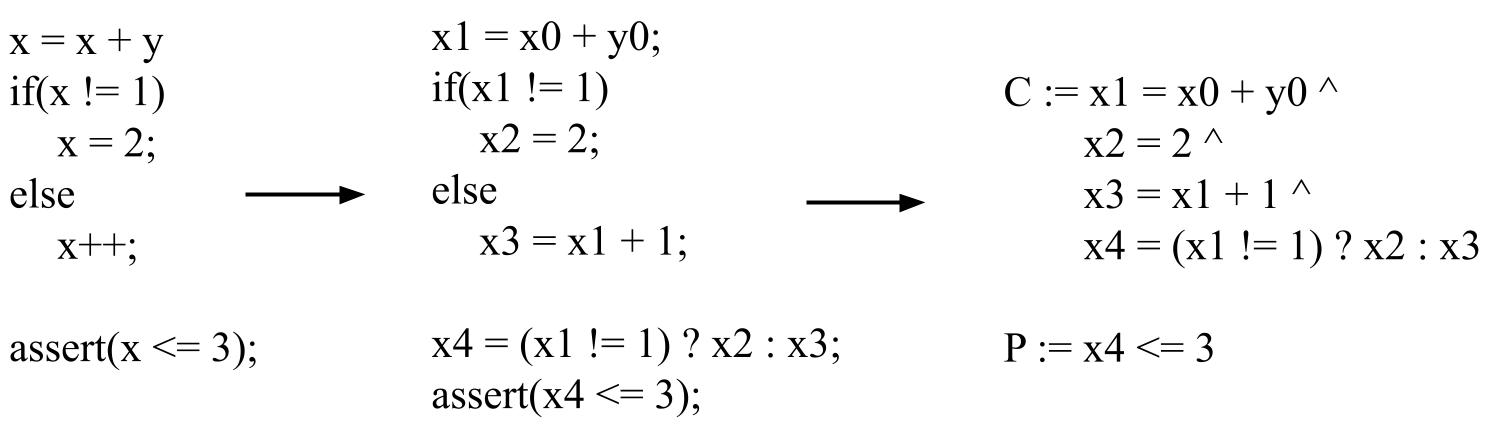
\includegraphics[width=0.75\textwidth]{code-conversion.jpg}
  \caption{Programa ejemplo transformado a SSA y fórmula}
  \label{fig: code-conversion}
\end{figure}

Dado un camino, los ciclos, si los hay, son desenrollados duplicando el cuerpo $n$ veces (para $n$ fijo).
Cada copia tiene un condicional que usa la misma condición que el ciclo por si requiere menos de $n$ iteraciones.
Luego de la última copia, se agrega una aserción que asegura que el programa nunca requiere más iteraciones.
Esta aserción usa la negación de la condición del ciclo (la llamamos aserción desenrollada) y nos permite saber si la cota es suficientemente larga para cubrir todos los ciclos.
Respecto a los goto y llamadas a funciones, estos se desenrollan de una forma similar \cite{tacas-2004}.

Posteriormente, este programa es transformado en una forma SSA (static single-assignment) de modo que cada variable sea asignada exactamente una vez, y para que 
los punteros se simulen como estados abstractos en función de las asignaciones que se le realicen (son tratados como funciones no interpretadas).
Se reemplazan las variables originales y construcciones por equivalentes con el mismo efecto pero que facilitarán la verificación \cite{cbmc-slides}.
Finalmente, gracias a ello se producen dos ecuaciones de vectores de bits: $C$ para las restricciones y $P$ para la propiedad.
Para corroborar esta propiedad, entonces, la fórmula buscada es $C \land \neg P$.

Una vez construida esta fórmula, se transforma en CNF usando el método de Tseytin y se pasa a un procedimiento de decisión (SAT/SMT) para obtener una asignación 
satisfactible que la verifique (es decir, que sea la traza de error).
El procedimiento de decisión que se requiere debe poder manejar lógica de vectores de bits, arreglos, listas, conjuntos y diccionarios \cite{cbmc-slides}.
Además, se sugiere usar un solucionador incremental SAT para reducir la complejidad de la fórmula a verificar, de modo que se añadan primero las partes fáciles 
de la fórmula y las complejas solo cuando sea necesario.

%
\section{Aplicaciones y Casos de Estudio}
CBMC es herramienta versátil y que provee una funcionalidad de verificación que permite ser utilizada tanto en el sector académico como en el industrial, e incluso
en el competitivo (como se podrá ver a continuación en nuestro caso de estudio presentado).
Además, el sector o área de estudio en el que se utiliza es de lo más diverso incluyendo sectores como verificación de programas concurrentes \cite{cbmc-concurrent}, 
hardware \cite{cbmc-hardware-case}, sistemas operativos \cite{cbmc-tinyos-case}, implementación de drivers \cite{cbmc-drivers-case} e incluso de
librerías de criptografía \cite{cbmc-ecc-case,cbmc-prng-case}; corroboración de equivalencia entre programas (o una simulación con un modelo) 
\cite{cbmc-equiv-code-generators-case,cbmc-equiv-stateflow-case}, análisis de sistemas físicos y de control \cite{cbmc-vehicles-case}, generación automática de vectores 
de prueba \cite{cbmc-testing-case1,cbmc-testing-case2}, cálculo del tiempo de ejecución en el peor caso (WCET) \cite{cbmc-wcet-case}, entre otros.
Otro sector en el que fue aplicado, más ajeno a la computación, es en biología para el estudio de restricciones del tráfico de vesículas en células eucariotas \cite{cbmc-biology-case}.

Como caso de estudio elegido para mostrar y reflejar el potencial y la utilidad de la herramienta, hemos decidido romper un cifrado customizado que consta 
de una sucesiva aplicación de una encriptación XOR con clave repetida (variante del cifrado de Vernam \cite{crypto-book}) como parte 
del reto ``XtraORdinary'' \footnote{``XtraORdinary''. Disponible en \url{https://play.picoctf.org/practice/challenge/208}. Accedido el 21 de mayo de 2025.}
propuesto en la competencia Capture The Flag ``picoMini'' en el año 2021.

Debido a que la importancia de esta sección reside en la utilización de CBMC, los aspectos técnicos y reducciones realizadas como parte del reto no se presentarán; 
sino que directamente se detallará la solución sobre la versión ya simplificada.
La versión completa junto con los archivos tanto del reto como de la solución se encuentra en el repositorio de este informe
\footnote{CBMC Analysis Report. Disponible en \url{https://github.com/helcsnewsxd/cbmc-analysis-report}}.

En la versión simplificada, el objetivo es quebrar un cifrado obteniendo el mensaje original que corresponde con el mensaje encriptado interceptado
de longitud $76$ (en formato hexadecimal):
\begin{verbatim}
            57657535570c1e1c612b3468106a18492140662d2f5-
                967442a2960684d28017931617b1f3637
\end{verbatim}

El algoritmo de cifrado aplica sucesivamente la encriptación XOR con clave repetida con $6$ palabras donde la primera a aplicar es una clave desconocida (privada)
mientras que las restantes $5$ son claves conocidas (públicas).
La encriptación con la clave privada siempre se realiza, pero con las públicas depende de un condicional sujeto a una condición aleatoria (es decir,
existen $2^5$ opciones de esquemas de cifrados posibles).

En base a ello, el uso de CBMC consta en la implementación del modelo de cifrado descripto con valores desconocidos para la flag (de longitud conocida igual 
a la mitad del mensaje interceptado: $38$), la clave (de longitud desconocida) y los $5$ condicionales que corresponden a la aplicación o no del encriptado para cada clave pública.
En este modelo se hace uso de la búsqueda de trazas de error generada por CBMC al colocar como aserción final que la bandera encriptada en el cifrado es distinta a la interceptada.
De este modo, esta traza muestra los estados correspondientes al par \texttt{(flag, key)} que generan el mismo valor interceptado.

Para reducir la búsqueda de posibles entradas que hagan fallar la aserción, se utiliza también la funcionalidad de contratos en código que CPROVER dispone en la herramienta CBMC.
En este caso particular, se hace uso de \verb|__CPROVER_assume()| para asegurar propiedades que tanto el mensaje original como la clave privada deben cumplir.
En particular, algunas de estas condiciones implican que ambas contienen solo caracteres imprimibles y que el formato de la bandera es \verb|picoCTF{...}|.

Finalmente, y debido a que el análisis devuelve una sola traza de error, para hacer más eficiente la búsqueda se desarrolló un script que ejecute el análisis por 
parte de esta herramienta para cada posible tamaño de la clave privada (entre $1$ y $38$), de modo que podamos obtener todos los pares de mensaje y clave originales posibles.
Gracias a esto, en $6.45$ segundos \footnote{Computadora con Sistema Operativo Windows 11 Pro 24H2, 16GB de RAM y procesador AMD Ryzen 7 5700G}, se pudo obtener 
el mensaje original y con ello romper este cifrado.
La bandera original es \verb|picoCTF{w41t_s0_1_d1dnt_1nv3nt_x0r???}|.

%
\section{Comparación con Otras Herramientas}
La comparación estará basada en el trabajo realizado por Dirk Beyer y Thomas Lemberger \cite{cbmc-comparison}.
En principio, se compara a CBMC junto con herramientas de testing tradicional (generadores de tests de código automáticos, por ejemplo) y
con otras herramientas de verificación formal (\textit{model checkers}).
Esta comparación no es trivial, ya que el testing tradicional es una forma de testing muy usada en muchos lenguajes, aunque con algunas desventajas en C.
Si bien en los trabajos se menciona que el rendimiento de verificadores formales como CBMC, es mucho mejor en comparación al testeo tradicional; los verificadores
entre sí tienen diversas mejoras que hacen que uno sea mejor que otro.

Comenzando por el testing tradicional, el mismo brinda una forma más accesible de testeo para desarrolladores (a veces los verificadores 
formales pueden parecer complejos si uno no tiene conocimiento en lógica formal).
También, permiten testear características específicas de nuestro programa manualmente.
En contraste, el testing tradicional no puede garantizar ausencia de errores (pero si la presencia).
Además, debido a la falta de estandarización para C, la generación de tests automáticos es muy difícil de llevar a cabo \cite{cbmc-comparison}, 
por lo que no son fácilmente escalables para programas complejos.
Por ambos motivos, aquí CBMC se posiciona como una mejor opción al poder garantizar ausencia de errores (respecto a una cota/límite) y debido a que es escalable a programas complejos.

Respecto a la comparación de CBMC con otros verificadores formales, se destacan que herramientas como CPA-Seq y ESBMC-incr tienen ventajas ante esta.
CPA-Seq combina técnicas más avanzadas que le permiten ser mucho mas profundo y rápido a la hora de explorar los caminos posibles de un programa.
Según la experimentación realizada en los estudios de D. Beyer y T. Lemberger, CPA-Seq encuentra un $59.66\%$ de errores mientras que CBMC un $55.7\%$. \cite{cbmc-comparison}

El otro verificador es ESBMC-incr, una variación de CBMC con algunas mejoras.
Entre ellas, aplica una variación del bounded model checking en el que se basa CBMC pero incremental (no fijo), lo cual es mucho mas exhaustivo a la hora de buscar errores.
En comparación con CBMC y CPA-Seq, ESBMC-incr encuentra $63.69\%$ de errores \cite{cbmc-comparison}, consolidándose como la mejor.

%
\section{Conclusión}
En este informe presentamos un análisis general de CBMC.
Abordamos su funcionamiento interno, su usabilidad desde la línea de comandos, sus aplicaciones en distintos dominios y su desempeño en comparación con otras herramientas.
Además, incluimos un caso de estudio en criptografía para evidenciar su versatilidad.

Su enfoque basado en Bounded Model Checking y las transformaciones que aplica para traducir código a su representación lógica para luego aplicar SAT/SMT solvers, la convierte
en una herramienta eficaz para la detección de errores comunes.
Además, no solo permite verificar propiedades estándares de seguridad, sino también que el usuario pueda definir aserciones personalizadas que considere
relevantes para el software específico que se esté analizando, lo cual amplía significativamente su aplicación.

Cabe destacar también su facilidad de uso desde la línea de comandos: las flags son directas y permiten configurar rápidamente distintos modos de análisis.
No es necesario descargar herramientas extras para su uso, y viene instalado por defecto en Linux, por lo que es fácil de acceder a la misma (en caso de Windows o MacOS, 
su instalación es muy simple).

Más allá de su uso tradicional en la verificación formal de software, CBMC ha demostrado ser útil en una variedad de dominios, desde la verificación de controladores en
sistemas embebidos hasta aplicaciones de criptografía o biología.
Esto queda evidenciado en el caso de estudio presentado en este informe.

En conclusión, CBMC no solo destaca por su eficiencia, si no también por su flexibilidad y lo accesible que es, lo que la convierte en una valiosa opción tanto para
proyectos de la academia como para industria.

\bibliographystyle{splncs04}
\bibliography{references}

\end{document}
